
\documentclass[submit]{harvardml}


\course{CS181-S19}
\assignment{Assignment \#4}
\duedate{11:59pm April 5, 2019}

\usepackage[OT1]{fontenc}
\usepackage[colorlinks,citecolor=blue,urlcolor=blue]{hyperref}
\usepackage[pdftex]{graphicx}
\usepackage{subfig}
\usepackage{fullpage}
\usepackage{amsmath}
\usepackage{amssymb}
\usepackage{color}
\usepackage{todonotes}
\usepackage{listings}
\usepackage{common}
\usepackage{bm}

\usepackage[mmddyyyy,hhmmss]{datetime}

\definecolor{verbgray}{gray}{0.9}

\lstnewenvironment{csv}{%
  \lstset{backgroundcolor=\color{verbgray},
  frame=single,
  framerule=0pt,
  basicstyle=\ttfamily,
  columns=fullflexible}}{}

\begin{document}
\begin{center}
{\Large Homework 4: Clustering and EM}\\
\end{center}


This homework assignment focuses on different unsupervised learning
methods from a theoretical and practical standpoint.  In Problem 1,
you will explore Hierarchical Clustering and experiment with how the
choice of distance metrics can alter the behavior of the algorithm. In
Problem 2, you will derive from scratch the full
expectation-maximization algorithm for fitting a Poisson mixture
model. In Problem 3, you will implement PCA on a dataset of
handwritten images and analyze the latent structure learned by this
algorithm.

There is a mathematical component and a programming component to this
homework.  Please submit your PDF, tex, and Python files to Canvas,
and push all of your work to your GitHub repository. If a question
requires you to make any plots, please include those in the writeup.

\newpage

\begin{problem}[Hierarchical Clustering, 7 pts]
  
At each step of hierarchical clustering, the two most similar clusters
are merged together. This step is repeated until there is one single
group. We saw in class that hierarchical clustering will return a
different result based on the pointwise-distance and cluster-distance
that is is used. In this problem you will examine different choices of
pointwise distance (specified through choice of norm) and cluster
distance, and explore how these choices change how the HAC algorithm
runs on a toy data set.

  
 Consider the following four data points in $\reals^2$, belonging to three clusters: the
  black cluster consisting of $\boldx_1 = (0.1, 0.5) $ and $\boldx_2 = (0.35, 0.75))$,
  the red cluster consisting of $\boldx_3 = (0.28, 1.35)$, and the blue cluster
  consisting of $\boldx_4 = (0, 1.01)$.

  \begin{center} 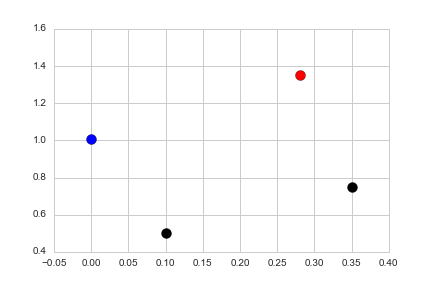
\includegraphics[scale=.3]{scatterplot.png} \end{center}


  Different pointwise distances $d(\boldx, \boldx') = \|\boldx - \boldx'\|_p$
  can be used.  Recall the definition of the
  $\ell_1$, $\ell_2$, and $\ell_{\infty}$ norm:
  \begin{eqnarray*}
     \| \mathbf{x} \|_1 = \sum_{j = 1}^m |x_i| \quad \quad\quad \| \mathbf{x} \|_2 = \sqrt{\sum_{j = 1}^m x_i^2 } \quad\quad\quad
     \| \mathbf{x} \|_{\infty} = \max_{j \in \{1, \ldots, m\}} |x_j|\\
  \end{eqnarray*}
  
  Also recall the definition of min-distance, max-distance,
  centroid-distance, and average-distance between two clusters (where $\bmu_{G}$
is the center of a cluster $G$):
%
\begin{eqnarray*}
    d_{\text{min}}(G, G') &=& \min_{\boldx  \in G, \boldx' \in G'} d(\boldx, \boldx')\\
    d_{\text{max}}(G, G') &=& \max_{\boldx  \in G, \boldx' \in G'} d(\boldx, \boldx')\\
    d_{\text{centroid}}(G, G') &=&  d(\bmu_{G}, \bmu_{G'})\\
    d_{\text{avg}}(G, G') &=&\frac{1}{|G| |G'|} \sum_{\boldx \in G}\sum_{\boldx'  \in G'} d(\boldx, \boldx')\\
  \end{eqnarray*}

  \begin{enumerate}
  \item Draw the 2D unit sphere for each norm,
  defined as $\mathcal{S} = \{\boldx \in \mathbb{R}^2: \|\boldx\| = 1 \}$. Feel free to do
  it by hand, take a picture and include it in your pdf.
\item  For each norm ($\ell_1, \ell_2, \ell_\infty$) and each clustering distance, specify which two clusters would
  be the first to merge.
\item Draw the complete dendrograms showing the order of agglomerations for the $\ell_2$ norm and each of the clustering distances. We have provided some code to make this easier for you. You are not required to use it.
  \end{enumerate}


\end{problem}

\subsection*{Solution}

\newpage 

\begin{problem}[Expectation-Maximization for Poisson Mixture Models, 7pts]

In this problem we will explore expectation-maximization for the
Poisson Mixture model.  Each observation $\boldx_n$ is a vector in the
non-negative integers $\mathbb{Z}^{*}$.  We posit that each
observation comes from \emph{one} mixture component.  For this
problem, we will assume there are $K$~components. Each component $k
\in \{1, \ldots, K\}$ will be associated with a mean vector $\lambda_k
\in R^{+}$.  Finally let the (unknown) overall mixing proportion of
the components be~$\btheta \in [0,1]^K$, where~${\sum_{k=1}^K
  \btheta_k=1}$.

Our generative model is that each of the~$N$ observations comes from a
single component.  We encode observation $n$'s component-assignment as
a one-hot vector~${\boldz_n \in \{0,1\}^K}$ over components. This
one-hot vector is drawn from~$\btheta$; then, $\boldx_n$ is drawn
from~$\text{Poisson}(\lambda_{z_n} )$, which simply means that if $\boldz_{nj} = 1$ for some $j \in \{1,\ldots, K\}$ (i.e. the $j$th element of $\boldz_n$ equals $1$), then $\boldx_n \sim \text{Poisson}(\lambda_j)$. 

Formally, documents are generated in two
steps:
\begin{eqnarray*}
 \boldz_n &\sim& \text{Categorical}(\btheta) \\
 \boldx_n &\sim& \text{Poisson}(\lambda_{z_n} )
\end{eqnarray*}

  \begin{enumerate}

  \item \textbf{Intractability of the Data Likelihood} We are
    generally interested in finding a set of parameters $\lambda_k$
    that maximize the data likelihood $\log p(\{\boldx_n\}^N_{n=1}|\{\lambda_k\}^K_{k = 1})$.
    Expand the data likelihood to include the necessary sums over
    observations $\boldx_n$ and latents $\boldz_n$.  Why is optimizing this loss
    directly intractable?
    
\item \textbf{Complete-Data Log Likelihood} Define the complete data for this problem to be $D = \{(\boldx_n, \boldz_n)\}_{n=1}^N$. Write out the complete-data negative log likelihood. Note that optimizing this loss is now computationally tractable if we know $\boldz_n$.

\[\mcL(\btheta, \{\lambda_k\}^K_{k=1}) =  -\ln p(D \given\btheta, \{\lambda_k\}^K_{k=1}).\] 
    

\item \textbf{Expectation Step}
Our next step is to introduce a mathematical expression for $\boldq_n$, the posterior over the hidden topic variables~$\boldz_n$ conditioned on the observed data $\boldx_n$ with fixed parameters, i.e $p(\boldz_n | \boldx_n; \btheta, \{ \lambda_k \}^K_{k=1})$.

\begin{itemize}
\item  \textbf{Part 3.A } Write down and simplify the expression for $\boldq_n$. 
\item  \textbf{Part 3.B } Give an algorithm for calculating $\boldq_n$ for all $n$, given the observed data~$\{\boldx_n\}^N_{n=1}$ and settings of the parameters~$\btheta$ and~$\{ \lambda_k,  \}^K_{k=1}$.

\end{itemize}

\item \textbf{Maximization Step}
Using the~$\boldq_n$ estimates from the Expectation Step, derive an update for maximizing the expected complete data log likelihood in terms of~$\btheta$ and~$\{ \lambda_k \}^K_{k=1}$.

\begin{itemize}
    \item \textbf{Part 4.A } Derive an expression for the expected complete-data log likelihood in terms of $\boldq_n$.
    \item \textbf{Part 4.B } Find an expression for $\btheta$ that maximizes this expected complete-data log likelihood. You may find it helpful to use Lagrange multipliers in order to enforce the constraint $\sum \theta_k = 1$. Why does this optimized $\btheta$ make intuitive sense?
    \item \textbf{Part 4.C } Apply a similar argument to find the values of $\{\lambda_k
      \}^K_{k = 1}$ that maximizes the expected complete-data log likelihood.
\end{itemize}

\item Suppose that this had been a classification problem, that is,
  you were provided the ``true'' categories $\boldz_n$ of each
  document, and you were going to perform the classification by
  inverting the provided generative model.  Could you reuse any of
  your inference derivations above?  
  
\end{enumerate}


  
\end{problem}

\subsection*{Solution}




\newpage

\begin{problem}[PCA, 15 pts]

For this problem you will implement PCA from scratch.  Using
\texttt{numpy} to call SVDs is fine, but don't use a third-party
machine learning implementation like \texttt{scikit-learn}.

We return to the MNIST data set from T3.  You have been given
representations of 6000 MNIST images, each of which are $28\times28$
greyscale handwritten digits. Your job is to apply PCA on MNIST, and
discuss what kinds of structure is found.  

As before, the given code loads the images into your environment as a
6000x28x28 array.

\begin{itemize}

\item Compute the PCA.  Plot the eigenvalues corresponding to the most significant 500
  components in order from most significant to least. Make another plot that describes the cumulative proportion of variance explained by the first k most significant components for values of $k$, 1 through 500. 
  How much variance is explained by the first 500 components?  Describe
  how the cumulative proportion of variance explained changes with k.  

\item Plot the mean image as well as the images corresponding the
  first 10 principle components.  How does images compare to the
  cluster centers from K-means?  Discuss any similarities and
  differences.

\item Compute the reconstruction error on the data set using the mean
  image as well as the first 10 principle components.  How does this
  error compare to running K-means and using the cluster centers as
  the reconstructions for each image?  Discuss any similarities and
  differences.  

\end{itemize}


As in past problem sets, please include your plots in this
document. (There may be several plots for this problem, so feel free
to take up multiple pages.)




\end{problem}
\subsection*{Solution}


\newpage

\begin{itemize}
    \item Name:
    \item Email:
    \item Collaborators:
    \item Approximately how long did this homework take you to complete (in hours):   
\end{itemize}


\end{document}
